% Build on the outline below.  Cite by using \citep{Author2016} to add a
% parenthetical citation; use \citet{Author2016} to get a textual cite like
% this: Author (2016). 

\section{Plot Interaction Terms}

It has been well known for over a decade that models containing multiplicative interaction terms require particular care in interpretation \citep[see, e.g.,][]{Golder2003, Braumoeller2004, Brambor2006, Kam2007}. Nevertheless, many political scientists struggle with interaction terms: improperly specified or interpreted interaction terms appear at the top of Nyhan's (\citeyear{Nyhan2015}) list of ``recurring statistical errors'' that reviewers should be sure to check for. %http://thepoliticalmethodologist.com/2015/12/04/a-checklist-manifesto-for-peer-review/

First, as \citet[71-72]{Brambor2006} wrote, in models with multiplicative interaction terms, constitutive terms should not be interpreted as unconditional or marginal effects because ``the coefficient on X only captures the effect of X on when Z is zero.'' 


Given this, in Table 1, the coefficient on ``Median Household Income (X)'' only captures the effect of ``Median Household Income (X)'' on ``Rejection of Meritocracy (Y)'' when ``GINI Index (Z)'' is zero. Similarly, the coefficient on ``GINI Index (Z)'' captures the effect of ``GINI Index (Z)'' on ``Rejection of Meritocracy (Y)'' when ``Median Household Income (X)'' is zero. In this sense, we cannot conclude that ``the estimates (of GINI Index) reveal that, among those with the lowest incomes, an increase in county inequality is associated with a significant increase in the probability of rejecting meritocracy'' \citep[334]{Newman, Johnston, and Lown2015a} because the lowest value of ``Median Household Income'' variable is not 0, but 1 \citep{Newman2015a, 332}. 

Second, more importantly, the statistical significance of the interaction term does not mean that X has substantive conditional effect on Y. The table itself does not give us the sufficient information because the marginal effect of X on Y should be interpreted with the substantively relevant values of the variable Z. Moreover, as \citet[74]{Brambor2006} demonstrated, we cannot calculate the standard errors from the typical results table using a little algebra. Thus, a figure as Figure 1 is needed to show the marginal effect of X and the corresponding standard errors. Figure 1 plots the coefficient estimates for county income inequality (GINI Index) at each of the nine levels of income in the Pew data. In spite of the statistical significance of the interaction term in Table 1 of the original paper, the confidence intervals of these estimates all cross zero. In other words, none are statistically significant. The conclusion of \citet[334]{Newman2015a} that this result ``reveals that among low-income citizens, those residing in highly unequal contexts are significantly more likely to reject meritocratic ideals than those in relatively equal contexts'' is therefore erroneous.

Actually, \citet[334]{Newman2015a} did the similar work to show the substantive conditional effect as Figure 2 of their paper. However, this graph is not only insufficient to show the substantive conditional effect, but also it is not reproducible. They indicate that Figure 2 ``plots the predicted probability of rejecting meritocracy across levels of county inequality for citizens at the 5th and 95th percentiles of household income'', but we could not obtain the same results using the variable ``Median Household Income'' that ranges from 1 to 9. This is because in their published replication data for the Model 1 (White Respondents) of Table 1, the range of the variable ``Median Household Income'' is oddly .21 to 1. In sum, the conditional effect is statistically significant only when the variable ``Median Household Income'' ranges from .21 to 1, which is substantively meaningless since there are no respondents with values of ``Median Household Income'' below 1. 




\begin{figure}[htbp] 
  \caption{Logit Coefficients of Local Income Inequality by Respondent Income: Table 1, Model 1, From Replication Data}
  \label{F:coef.t1m1}
  \begin{center}
    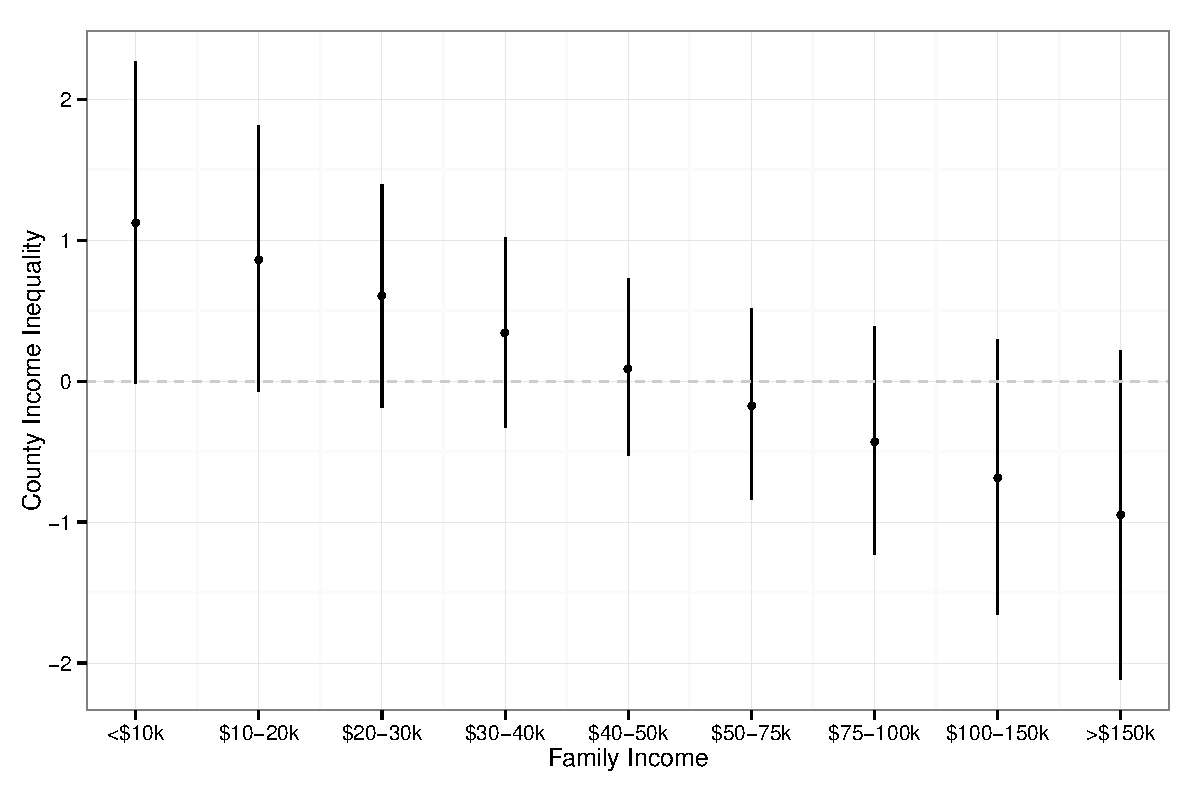
\includegraphics[width=5.25in]{../figures/07_plot_interaction_terms_t1m1.pdf}
  \end{center}
  \begin{footnotesize}
  \begin{tabular}{p{.1in} p{5.1in}}
  & \emph{Notes}: The coefficient for county income inequality fails to reach statistical significance for any observed level of respondent family income.
  \end{tabular}
  \end{footnotesize}
\end{figure}


% \begin{figure}[htbp] 
%   \caption{Logit Coefficients of Local Income Inequality by Respondent Income, Table B1, White Respondents, From Source Data with Missing Values Multiply Imputed}
%   \label{F:coef.b1m1}
%   \begin{center}
%     \includegraphics[width=5.25in]{../figures/07_plot_interaction_terms_b1m1_mi.pdf}
%   \end{center}
%   \begin{footnotesize}
%   \begin{tabular}{p{.1in} p{5.1in}}
%   & \emph{Notes}: The coefficient for county income inequality fails to reach statistical significance for any observed level of respondent family income.
%   \end{tabular}
%   \end{footnotesize}
% \end{figure}

